\setlength{\columnsep}{3pt}
\begin{flushleft}

	\begin{itemize}
		\item Logical partitions are partitions created inside the extended partition.
		\begin{figure}[h!]
			\centering
			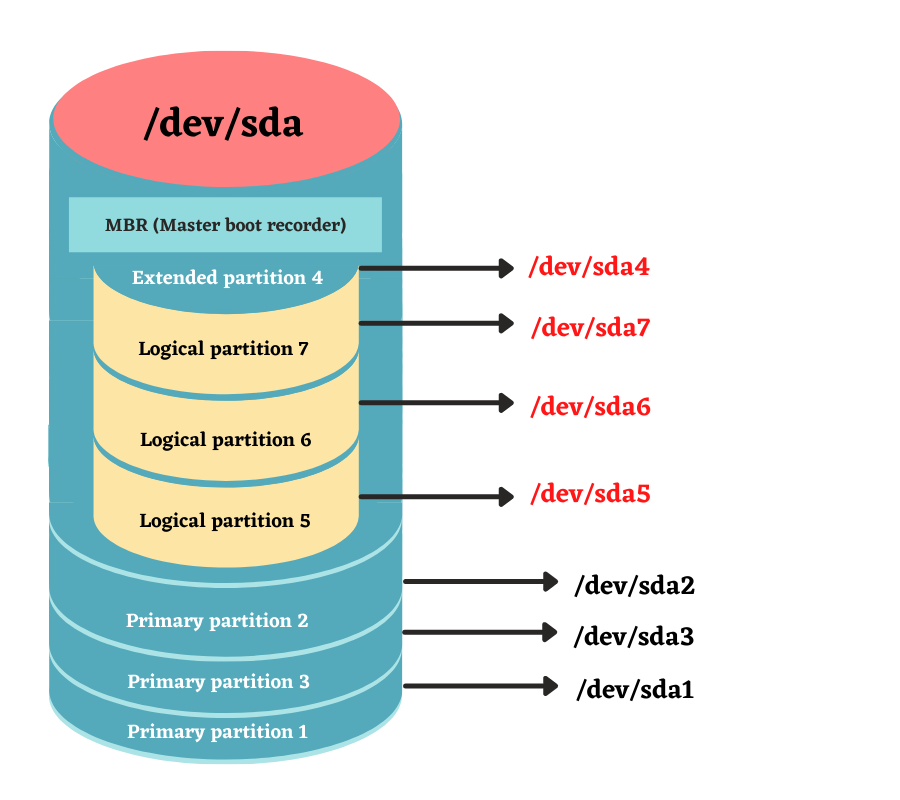
\includegraphics[scale=.6]{content/chapter8/images/logical.png}
			\caption{Logical partitions}
			\label{logical_naming}
		\end{figure}		
		
		\begin{tcolorbox}[breakable,notitle,boxrule=-2pt,colback=yellow,colframe=yellow]
			\color{black}
			Note: 
			\begin{itemize}
				\item Number of logical partitions is unlimited
				\item However, linux imposes limit on the total number of partitions on a drive
				\item There can be total 15 partitions on an SCSI disk and 63 total on an IDE disk
			\end{itemize}
		\end{tcolorbox}
		
	\end{itemize}


\newpage

\paragraph{fdisk command option to create logical partition}

\begin{itemize}
	\item \textbf{l}: Create a logical partition
\end{itemize}

Eg:
\begin{figure}[h!]
	\centering
	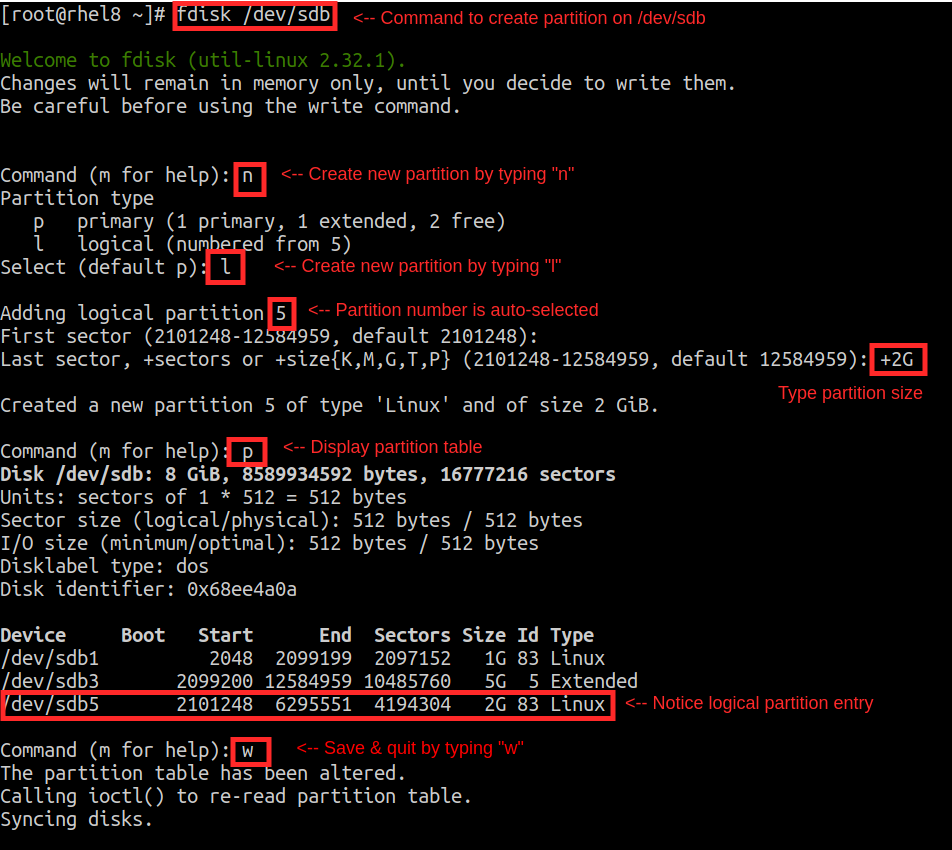
\includegraphics[scale=.4]{content/chapter8/images/logi.png}
	\caption{Creating logical partition}
	\label{primary_logi4}
\end{figure}		

\newpage

\paragraph{fdisk command option to delete any partition}

\begin{itemize}
	\item \textbf{d}: Delete partition
\end{itemize}
Eg:
\begin{figure}[h!]
	\centering
	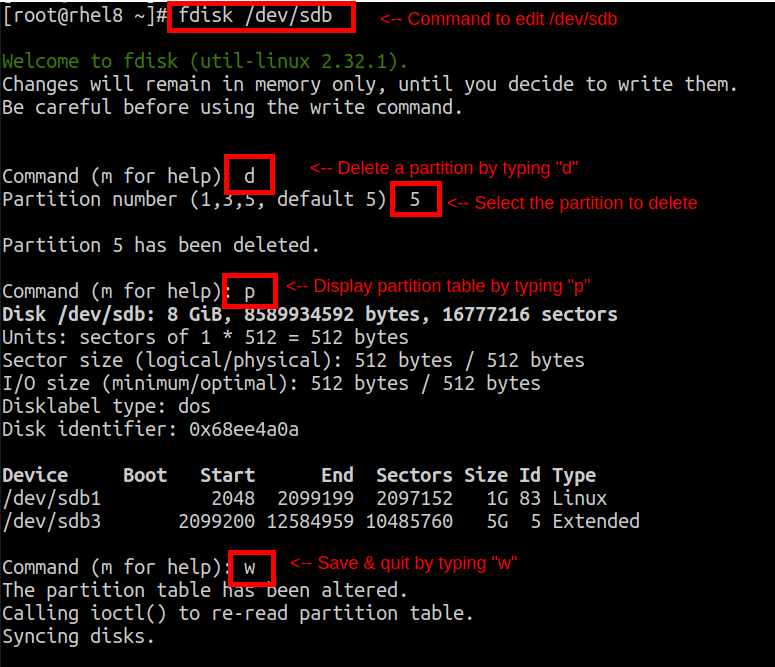
\includegraphics[scale=.4]{content/chapter8/images/delete.png}
	\caption{Deleting partition}
	\label{primary_logi3}
\end{figure}		



	
\end{flushleft}

\newpage

